%!TEX TS-program = xelatex
%!TEX encoding = UTF-8 Unicode
\documentclass[a4paper]{report}
%\usepackage[date=short,backend=biber]{apa}
\usepackage[hidelinks]{hyperref}
\usepackage{apacite}
\usepackage[dutch]{babel}
\usepackage[a4paper, left=1in, right=1in, top=1in, bottom=.8in]{geometry}
\usepackage[utf8]{inputenc}
\usepackage{fancyhdr}
\usepackage{nameref}
\usepackage{helvet}
\usepackage{titlesec}
\usepackage{geometry}
\usepackage{ragged2e}
\usepackage{graphicx}
\usepackage{etoolbox}
\usepackage{listings}
\usepackage{xspace}
\usepackage{xcolor}
\usepackage{nameref}
\usepackage{tcolorbox}
\usepackage{textcomp}
\usepackage[printonlyused,withpage]{acronym}
%%% Je mag zelf PWM implemetneren bij bijv peltierelement of het verwarming relais.

% Styling
\renewcommand{\rmdefault}{\sfdefault}
\pagestyle{fancy}
\patchcmd{\chapter}{\thispagestyle{plain}}{\thispagestyle{fancy}}{}{}

\fancyhf{}
\fancyhead[L]{ \turtleguard }
\fancyhead[R]{ Projectplan }
\fancyfoot[R]{\thepage}

\titleformat{\chapter}[hang]
{\normalfont\huge\bfseries}{\thechapter.}{10pt}{\huge}
\titlespacing{\chapter}{0pt}{-30pt}{20pt}

\setlength{\parindent}{0.2em}

\textwidth=400pt
\geometry{
    left=25mm
}

\renewcommand{\contentsname}{Inhoudsopgave}
%\RaggedRight % Don't 'block-justify' text

\definecolor{codegreen}{rgb}{0,0.6,0}
\definecolor{codegray}{rgb}{0.5,0.5,0.5}
\definecolor{codepurple}{rgb}{0.58,0,0.82}
\definecolor{backcolour}{rgb}{0.95,0.95,0.92}

\lstdefinestyle{mystyle}{
    backgroundcolor=\color{backcolour},   
    commentstyle=\color{codegreen},
    keywordstyle=\color{magenta},
    numberstyle=\tiny\color{codegray},
    stringstyle=\color{codepurple},
    basicstyle=\ttfamily\footnotesize,
    breakatwhitespace=false,         
    breaklines=true,                 
    captionpos=b,                    
    keepspaces=true,                 
    numbers=left,                    
    numbersep=5pt,                  
    showspaces=false,                
    showstringspaces=false,
    showtabs=false,                  
    tabsize=2
}

\lstset{style=mystyle}



% Commands
\newcommand{\teambox}{
  \begin{tcolorbox}[hbox, colback=blue!5!white,colframe=blue!75!black,
    left=.1mm, right=.1mm, top=.1mm, bottom=.1mm, fontupper=\scriptsize\sffamily]
    Team Keuze
  \end{tcolorbox}
}

\newcommand{\personalbox}{
  \begin{tcolorbox}[hbox, colback=green!5!white,colframe=green!75!black,
    left=.1mm, right=.1mm, top=.1mm, bottom=.1mm, fontupper=\scriptsize\sffamily]
    Persoonlijke Keuze
  \end{tcolorbox}
}
\newcommand{\teamchoice}[1]{
  \section[ #1 ]{#1~\mbox{\teambox}}
}

\newcommand{\personalchoice}[1]{
  \section[ #1 ]{#1~\mbox{\personalbox}}
}
\newcommand{\turtleguard}{\mbox{TurtleGuard\texttrademark}\xspace}

% Document
\begin{document}


% Title Page
\begin{titlepage}
    \begin{center}
        \vspace*{.9cm}
        \Huge
        \textbf{ Projectplan \turtleguard }\\
        \vspace{0.2cm}
        \small\textit{"Hét ultieme schild-bad voor jouw schildpad"}

        \normalsize


        
        
\includegraphics[width=0.7\textwidth]{Images/turtleguard.png}
        \vspace{1cm}
        \Large\\
        \textbf{Mede mogelijk gemaakt door} \\
        
\includegraphics[width=0.2\textwidth]{Images/logouni.png}


        \vfill
      \end{center}
        \textbf{Student:} Vincent van Setten - 1734729 \\
        \textbf{Opdrachtgever:} HU University of Applied Sciences\\
        \textbf{Datum:} \today \\
        \vspace{2cm}
\end{titlepage}


% ToC
\tableofcontents

\chapter*{Versiebeheer}
\thispagestyle{empty}  % Removes header and footer from this specific page
\begin{table}[h]
    \centering
    \begin{tabular}{|c|c|c|p{5cm}|}
        \hline
        Versie & Datum      & Changes Made  \\
        \hline
        1.0    & 2023-09-10 & Eerste Versie \\
        \hline
    \end{tabular}
    \caption{Versiebeheer}
\end{table}
\clearpage  % End of the page

\chapter{Algemene Informatie}
\section{Introductie}
Dit document dient als project- en testplan voor het \turtleguard systeem. Het \turtleguard systeem wordt verder in detail besproken in hoofdstuk \ref{section-product}.
Verdere hoofdstukken beschrijven de architectuur van het product, de eisen aan het product en de tests die uitgevoerd zullen worden.
Het uiteindelijke doel van dit document is het beschrijven van een regelsysteem, in dit geval \turtleguard, welke ten minste twee sensoren en actuatoren bevat. 

\section{Productomschrijving}
\label{section-product}
Huisdieren, we zijn er (bijna) allemaal gek op. Vanzelfsprekend is het dus dat we het onze vertrouwde gezelschap zo comfortabel mogelijk willen maken.
Bij de meeste huisdieren is het relatief simpel, \mbox{zoals} bij een kat of hond. Zorg voor eten, drinken en aandacht en dan zijn ze vaak wel tevreden.
\par \smallskip
Helaas is het niet bij alle huisdieren zo eenvoudig. 
Zo heeft bijvoorbeeld een muskus schildpad best strenge eisen aan het water: naast het voeren, moeten bijvoorbeeld ook de temperatuur en de \mbox{pH-waarde} van het water precies goed zijn.  
Als mens kunnen wij dit niet altijd even eenvoudig controleren. \par \smallskip 

Daarom stellen wij voor: \turtleguard.
Dit systeem hanteert een specifieke temperatuur voor uw \mbox{waterschildpad} en laat u weten als de waterkwaliteit niet aan de eisen voldoet.
Met \turtleguard hoeft u zich nooit meer druk te maken of uw schildpad zich wel comfortabel voelt in zijn schild.

\section{Kwaliteitscriteria}

\section{Begrippen}
\begin{acronym}
\acro{TDS}{Total Dissolved Solids}
\acro{ppm}{Parts Per Million}
\end{acronym}

\chapter{Systeem Architectuur}
\section{Hardware}


\subsection{Sensoren}
Ik ga gebruik maken van drie verschillende sensoren. Mijn keuzes en het gebruik van deze sensoren licht ik hieronder toe.
Dit zijn de sensoren die ik ga gebruiken.
\begin{itemize}
  \item EZO\texttrademark \space pH Circuit (pH meter)
  \item EZO\texttrademark \space Conductivity Circuit (TDS Sensor)
  \item DS18B20 (Water Thermometer)
  \item Adafruit MCP9808 (Lucht Thermometer)
\end{itemize}

\subsubsection{pH meter}
\paragraph{Gebruik} 
Een pH meter wordt gebruikt om de zuurgraad van het water te meten. 
Voor mijn schildpad is een pH van ongeveer 6.5 tot 7.5 nodig. 

\paragraph{Keuze} 
Om de pH digitaal te kunnen meten, heb ik gekozen voor de  EZO\texttrademark \space pH Circuit. 
Deze sensor is goed beschikbaar en kan gebruikt worden op 3.3v en 5v. De sensor zelf is verbonden met een breakout board, welke weer verbonden kan worden met een enkele data pin, wat het uitlezen erg eenvoudig maakt.

\subsubsection{TDS Sensor}
Een manier om kwaliteit van het water te testen, is het meten van deeltjes die in water oplosbaar zijn.
Dit heet \ac{TDS}. Als de TDS waarde te hoog is, moet het water vervangen worden. 
De ideale TDS ligt tussen de 125ppm en 300ppm. 

\subsubsection{Water Thermometer}
De thermometer houdt de temperatuur van het water bij. Als het water te koud is, wordt het verwarmt. Als het water te warm is, wordt het verkoeld.
De ideale temperatuur voor de muskus schildpad is ongeveer 25 \textdegree c. Het water mag zo'n 3 \textdegree c warmer of kouder zijn.

% Wss onnodig...
\subsubsection{Omgeving Thermometer}
Ook is er een thermometer voor de temperatuur van de omgeving. Deze wordt gebruikt om te controleren hoe warm of koud het is in de omgeving. Hiermee kunnen we kijken of we verwachten dat het water warmer of kouder gaat worden.
Als het bijvoorbeeld 35 \textdegree c is, zal het waarschijnlijk niet nodig zijn om het water te verwarmen. Als het daarentegen 15 \textdegree c is, zal het verkoelen van het water weer onnodig zijn.

Deze zal worden gebruikt in combinatie met de water temperatuur. Als bijvoorbeeld de omgevingstemperatuur 30 \textdegree c is en het water is 29 \textdegree c, zal het verwarmingselement uit moeten blijven totdat de omgevingstemperatuur weer onder de 25 \textdegree c zakt. Tot die tijd zal verkoeling nodig zijn tot het water temperatuur rond de 25 \textdegree c is.


\subsection{Actuatoren}
Binnen het project ga ik gebruik maken van een aantal actuatoren, welke worden aangestuurd door de boven genoemde sensoren.
De actuatoren zal ik hieronder verder toelichten. Ik ga de volgende actuatoren gebruiken voor mijn systeem.
\begin{itemize}
  \item Peltier element geschakeld met PWM dmv een relais
  \item Verwarmingselement, geschakeld met een relais (Exo Terra Turtle Heater(50w).)
  \item LED 
\end{itemize}

\subsubsection{Peltier Element}
Het peltier element wordt gebruikt om het water te verkoelen. 
Dit zal vooral nodig zijn op tropische zomerdagen, om het water koel genoeg te houden op een temperatuur van 25 \textdegree c.
Om het verkoelen rustig en accuraat te laten verlopen, ga ik hem schakelen met een relais, aangesloten op een PWM signaal.

\subsubsection{Verwarmingselement}
Op de meeste dagen zal het water te koud zijn voor de schildpad. Daarom is er een verwarmingselement nodig. 
Dit element regelt zelf het verwarmen van een water met een vooraf ingestelde temperatuur. 
Deze wordt ook geschakeld met een relais, zodat het water niet verwarmd blijft worden tijdens het afkoelen.

Ik ga gebruik maken van de Exo Terra Turtle Heater(50w).
Deze houdt het water standaard al op 25 \textdegree c. 

\subsubsection{LED}
Als laatste hebben we een simpele LED als actuator. Deze gaat branden om aan te geven dat het water niet van voldoende kwaliteit is.
Hiermee kan de eigenaar het water vervangen, zodra het nodig is. 

\subsection{Diagrammen}

\begin{figure}[h]
  \centering
  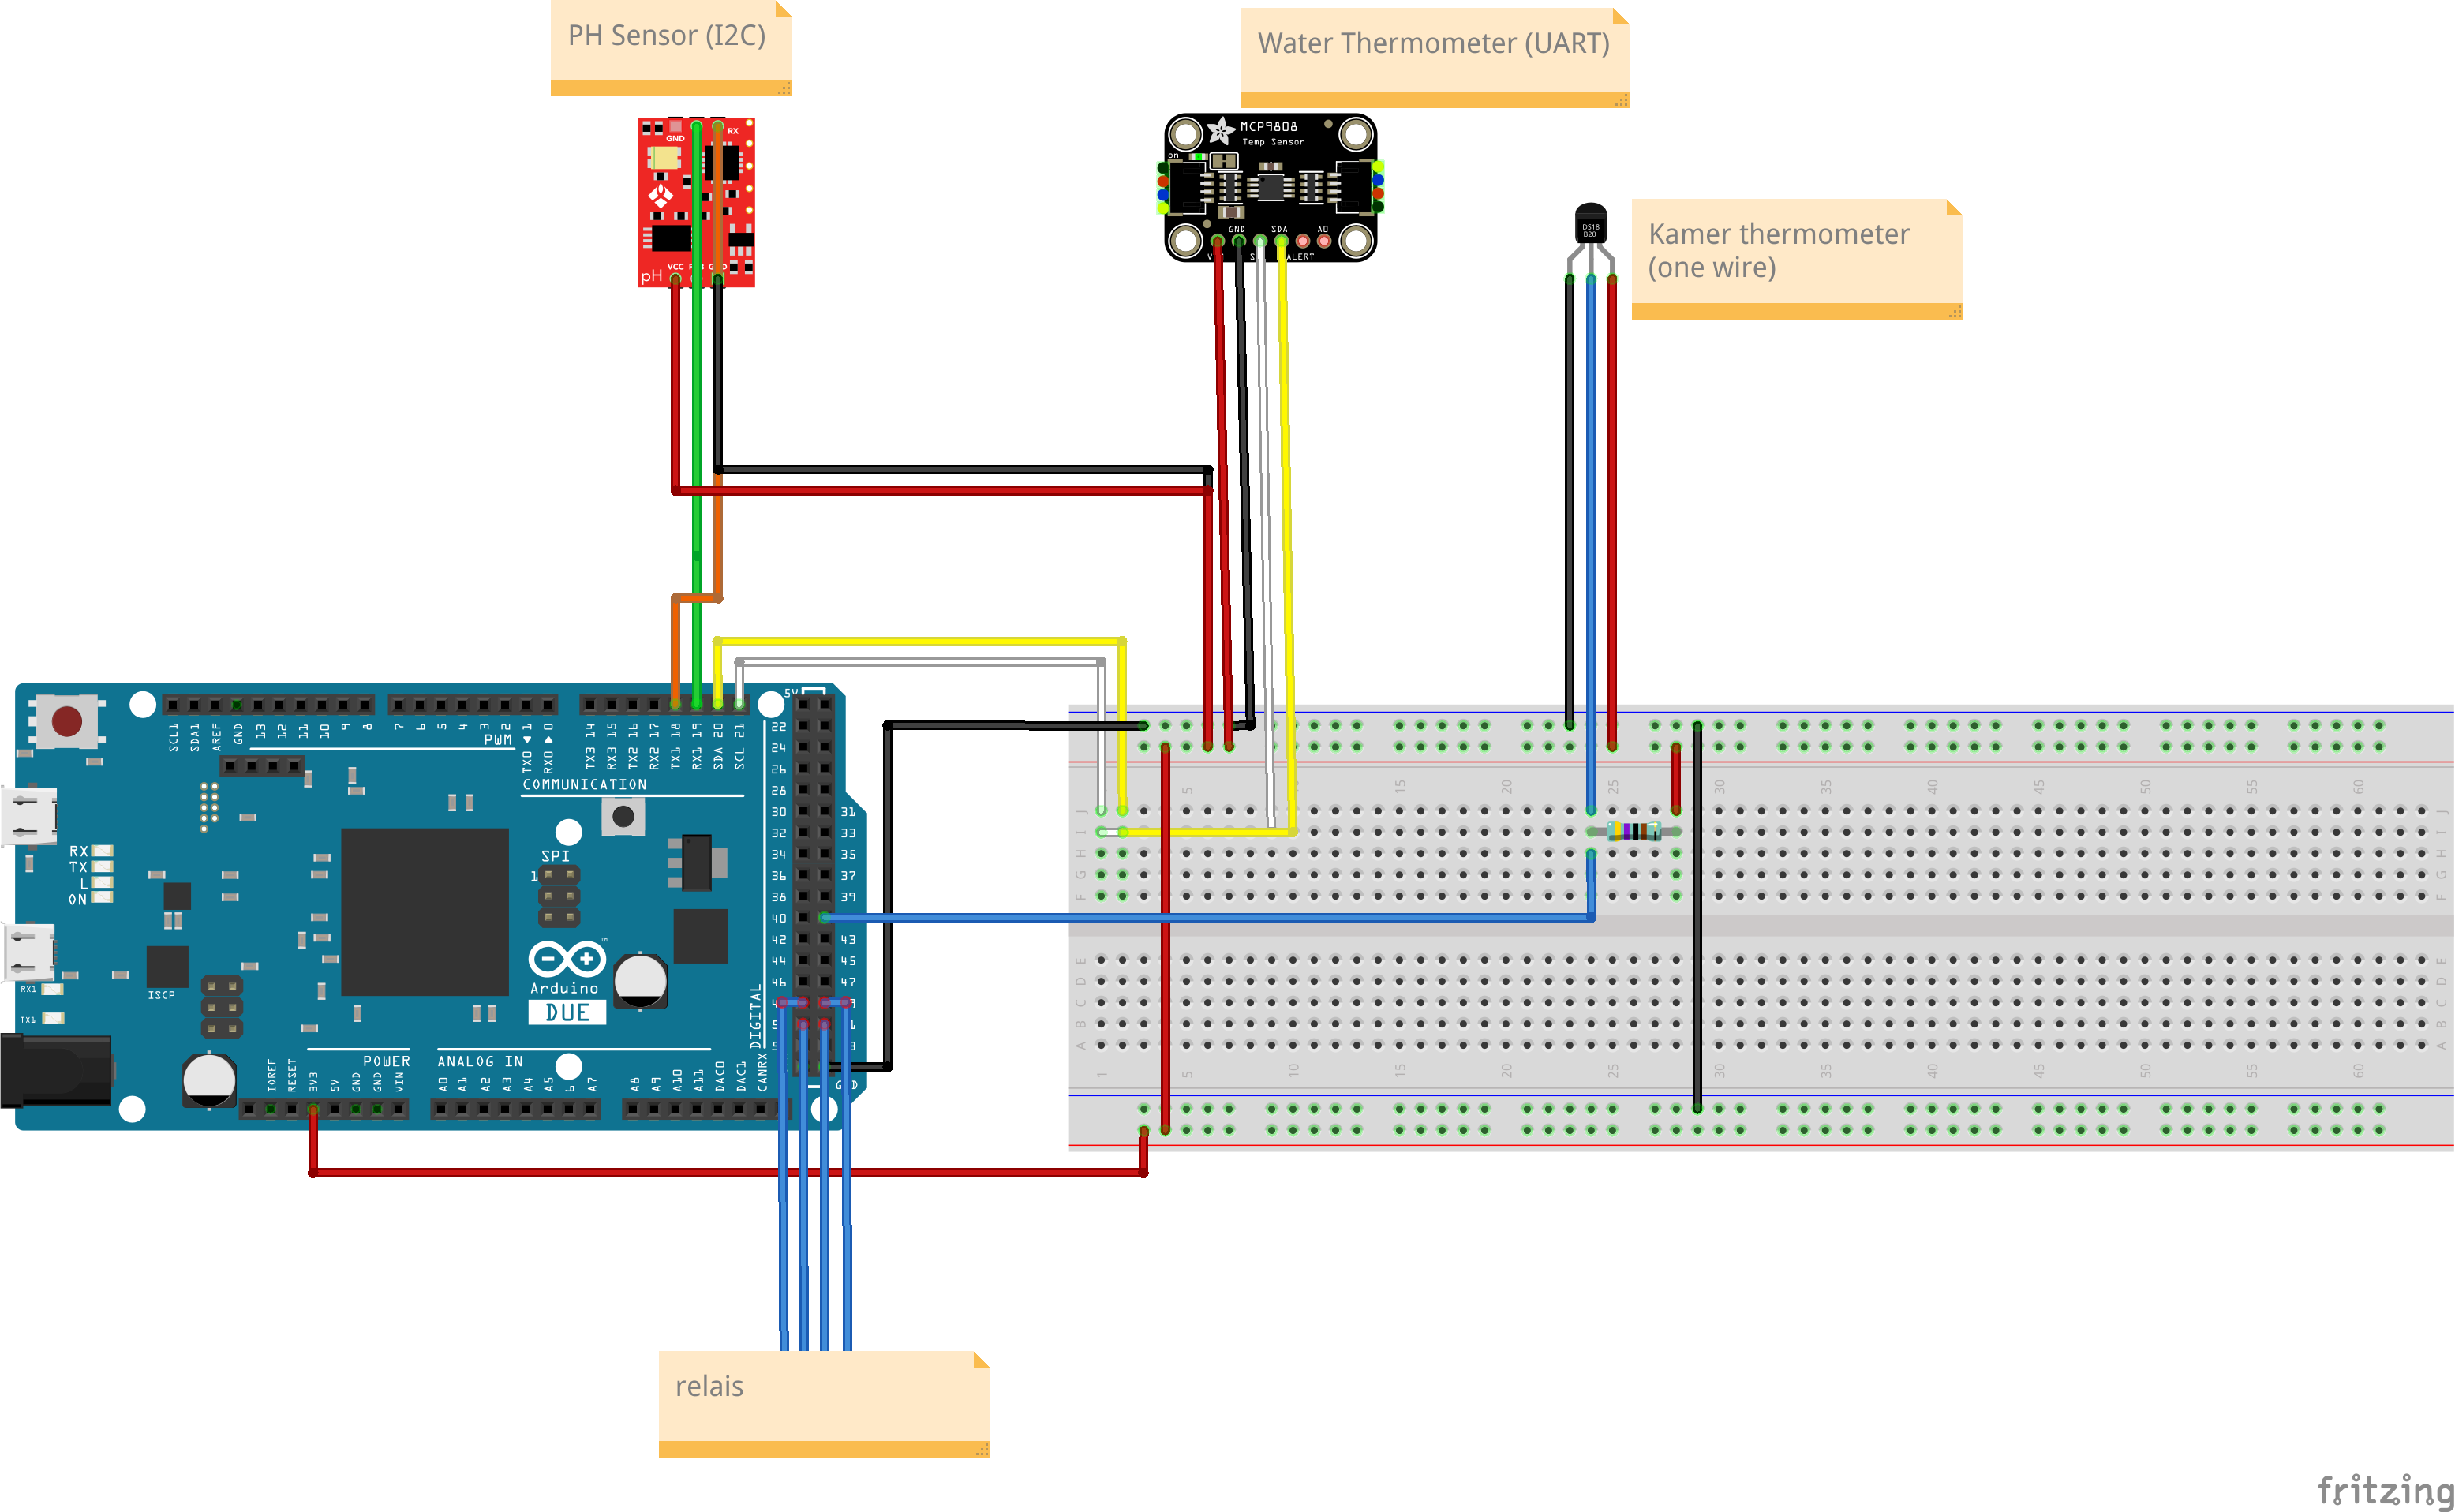
\includegraphics[width=0.9\textwidth]{Images/hardware_sketch_fritzing.png}
  \caption{Fritzing Hardware Diagram}
  \label{fig:hardware_sketch_fritzing}
\end{figure}
% TODO: Korte beschrijving over het diagram.

\section{Software}


\chapter{Testplan}
\section{Unit Tests}
\section{Integratietests}
\section{Systeemtests}
\section{Risicoanalyse}


\chapter{Bibliografie}
\nocite{*} % This includes all entries from the .bib file, even if they're not cited in the document
\begingroup
\renewcommand{\chapter}[2]{} % Removes the 'Chapter' heading
\renewcommand{\addcontentsline}[3]{} % Prevents adding this specific entry to TOC
\bibliographystyle{apacite}
\bibliography{bronnen}
\endgroup

\chapter{Bijlagen}

\end{document}